%!TEX root = ../main.tex

\section{Intervallschätzer - Konfidenzintervalle}
Die Intervallschätzer geben ein Intervall an, in dem sich der zu schätzende Parameter höchstwahrscheinlich befindet. Hierbei sind möglichst kleine Intervalle bei einer hohen Sicherheit natürlich gewünscht, aber diese Einschränkungen widersprechen sich. 
Verkleinert man das Intervall wird die Sicherheit, dass der geschätze Parameter wirklich enthalten ist im Allgemeinen kleiner.

Wir möchten nun zum Beispiel herausfinden, wie sicher wir uns sind, dass das Ergebnis eines Punktschätzers stimmt. Dafür bestimmen wir das \emph{Vertrauens- bzw. Konfidenzintervall}
\begin{equation*}
	J_n\coloneqq [\theta_u(X),\theta_o(X)]
\end{equation*}
wobei wir den Parameter $\theta$ schätzen, der Werte aus $\Theta$ annimmt. Die Zufallsvariablen 
\begin{equation*}
	\theta_u(X),\theta_o(X): \Omega\rightarrow \Theta
\end{equation*}
stellen dabei die untere und die obere Intervallgrenze dar. Sie beschreiben einen Grenzwert von $\theta$ in Abhängigkeit von der Stichprobe.

Dieses Intervall $J_n$ soll das unbekannte $\theta$ mit einer \emph{Garantiewahrscheinlichkeit} von $(1-\alpha)$ enthalten, das heißt
\begin{equation*}
	P_\theta (\theta\in J_n)=P_\theta(\theta_u(X)\leq \theta\leq \theta_o(X))\geq (1-\alpha)
\end{equation*}
für alle Werte des Parameters $\theta$.

\subsection{Abschätzen mit der Tschebyscheff-Ungleichung}
Eine grobe Abschätzung dieser Grenzen kann zum Beispiel über die \hyperref[tschebyscheff]{Tschebyscheff-Ungleichung} erfolgen.
Damit kann man die Wahrscheinlichkeit, dass der Parameter außerhalb des Intervalls liegt
\begin{equation*}
	P_\theta(|X-\theta|\geq \epsilon)\leq \frac{V(X)}{\epsilon^2}= \alpha
\end{equation*}
beschränken.
Es ergibt sich mit der Umformung 
\begin{equation*}
	\frac{V(X)}{\epsilon^2}= \alpha \quad \Leftrightarrow \quad \epsilon =\sqrt{\frac{V(X)}{\alpha}}
\end{equation*}
die Abschätzung für die beiden Intervallgrenzen
\begin{align*}
	\theta_u(X)&=X-\sqrt{\frac{V(X)}{\alpha}}\\
	\theta_o(X)&=X+\sqrt{\frac{V(X)}{\alpha}}.
\end{align*}
Diese garantiert für alle $\theta\in\Theta$, dass der unbekannte Parameter $\theta$ nur mit Unsicherheit $\alpha$ außerhalb des geschätzten Intervalls liegt.
\begin{equation*}
	P_\theta(p\not\in J_n)=\textstyle P_\theta\left(p\not\in \left[ X-\sqrt{\frac{V(X)}{\alpha}},X+\sqrt{\frac{V(X)}{\alpha}}\right]\right)\leq \alpha.
\end{equation*}


\subsection{Abschätzen über die Verteilungsfunktion}
Die Ergebnisse, die man durch die Abschätzung mit Tschebyscheff erhält, sind sehr grob. Einen genaueren Ansatz bietet die Abschätzung der Intervallgrenzen über die Verteilungsfunktion.

Wir betrachten dies anhand des Beispiels $X\sim\binomial(n,\theta)$, wobei $\theta$ wiederum unbekannt ist.

Wir wollen die beiden Konfidenzgrenzen $\theta_u(X),\theta_o(X)$ so bestimmen, dass gilt
\begin{equation*}
	P_\theta(\theta_u(X) \leq \theta )\geq 1-\beta \enspace\text{ und }\enspace P_\theta(\theta \leq \theta_o(X) )\geq 1-\beta.
\end{equation*}
Das heißt wir beschränken das Intervall von oben und unten jeweils mit der Konfidenzwahrscheinlichkeit $\beta=\frac\alpha2$.

Sei $k\in X(\Omega)$, $P_\theta(X\leq k)$ ist monoton fallend, wir bestimmen damit ein $\theta_u(k)$ und ein $\theta_o(k)$ so, dass gilt
\begin{equation*}
	P_{\theta_o(k)}(X\leq k)=\beta\enspace \text{ und }\enspace P_{\theta_u(k)}(X\leq k)=1-\beta.
\end{equation*}
Das heißt, wenn $\theta$ die obere Schranke wäre, ist die Wahrscheinlichkeit, dass $X$ kleinere Werte als $k$ annimmt genau $\beta$




\paragraph{?}
\begin{center}
	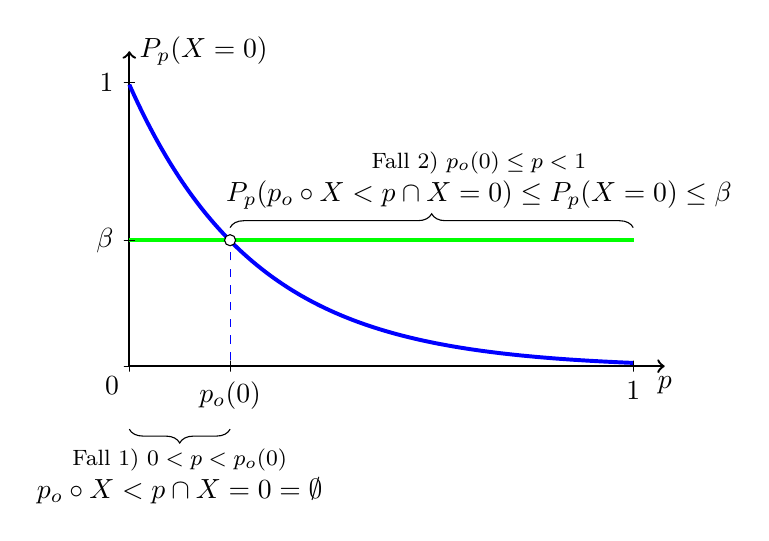
\begin{tikzpicture}[scale=0.8]
		\draw[->, line width=0.3mm] (0,0) to (8.5,0) node[below] {$p$};
		\draw[->, line width=0.3mm] (0,0) to (0,5) node[right] {$P_p(X=0)$};

		\draw[line width=0.5mm,scale=1,domain=0:8,smooth,variable=\x,blue, samples=100] plot ({\x},{4.5*exp(-0.5*\x)-0.03});

		\draw[line width=0.5mm,scale=1,domain=0:8,smooth,variable=\x,green, samples=100] plot ({\x},{2});	

		\draw (0,2) node (beta) [rectangle,inner sep = 0pt,minimum size = 0pt,minimum width=4pt,draw, label={left:$\beta$}] {};
		\draw (1.6,2) node (Pbeta) [fill = white,circle,inner sep = 0pt,minimum size = 4pt,draw] {};

		\draw (1.6,0) node (po) [rectangle,inner sep = 0pt,minimum size = 0pt,minimum height=4pt,draw, label={below:$p_o(0)$}] {};

		\draw[dashed, blue] (po) -- (Pbeta);
		
		\draw (0,0) node [rectangle,inner sep = 0pt,minimum size = 0pt,minimum height=4pt,draw, label={below left:$0$}] {};
		\draw (0,0) node [rectangle,inner sep = 0pt,minimum size = 0pt,minimum width=4pt,draw] {};
		
		\draw (8,0) node [rectangle,inner sep = 0pt,minimum size = 0pt,minimum height=4pt,draw, label={below:$1$}] {};

		\draw (0,4.5) node [rectangle,inner sep = 0pt,minimum size = 0pt,minimum width=4pt,draw, label={left:$1$}] {};


		\draw [decorate,decoration={brace,amplitude=5pt},yshift=0pt]
		(1.6,-1) -- (0,-1) node [black,midway,yshift=-0.6cm, align=center] 
		{\footnotesize Fall 1) $0<p<p_o(0)$\\$\simpleset{p_o\circ X< p}\cap\simpleset{X=0}=\emptyset$};


		\draw [decorate,decoration={brace,amplitude=5pt},yshift=0pt]
		(1.6,2.2) -- (8,2.2) node [black,midway,yshift=0.6cm, xshift=0.6cm, align=center] 
		{\footnotesize Fall 2) $p_o(0)\leq p<1$\\$P_p(\simpleset{p_o\circ X< p}\cap\simpleset{X=0})\leq P_p(X=0)\leq \beta$};
	\end{tikzpicture}	
\end{center}


\subsection{Approximation über die Normalverteilung}
Für große $n$ wird in der Praxis oft auf die Normalverteilung zurückgeführt und das Problem auf eine Quantilsbestimmung reduziert.

\begin{center}
	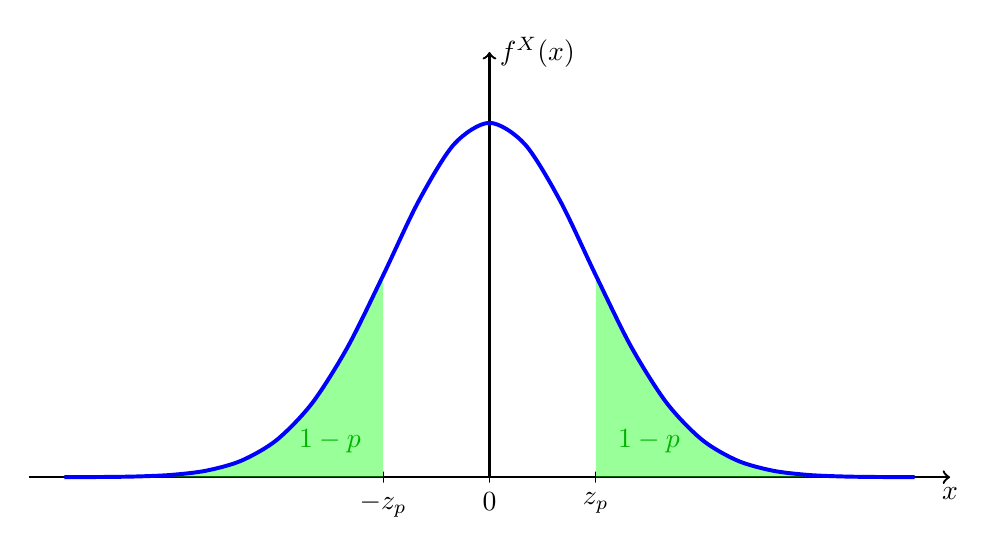
\begin{tikzpicture}[scale=0.9]
		\draw[->, line width=0.3mm] (-6.5,0) to (6.5,0) node[below] {$x$};
		\draw[->, line width=0.3mm] (0,0) to (0,6) node[right] {$f^X(x)$};

		\filldraw[scale=1,domain=-6:-1.5,smooth,variable=\x,fill=green, opacity=0.4, draw=none] plot ({\x},{5*exp(-\x*\x/4)}) -- (-1.5,0);
		\filldraw[scale=1,domain=1.5:6,smooth,variable=\x,fill=green, opacity=0.4, draw=none] plot ({\x},{5*exp(-\x*\x/4)}) -- (1.5,0);
		
		\draw[line width=0.5mm,scale=1,domain=-6:6,smooth,variable=\x,blue] plot ({\x},{5*exp(-\x*\x/4)});

		\draw (1.5,0) node (zp) [rectangle,inner sep = 0pt,minimum size = 0pt,minimum height=4pt,draw, label={below:$z_p$}] {};
		\draw (-1.5,0) node (-zp) [rectangle,inner sep = 0pt,minimum size = 0pt,minimum height=4pt,draw, label={below:$-z_p$}] {};

		\draw (-2.25,0.5) node[green!70!black] {$1-p$};
		\draw (2.25,0.5) node[green!70!black] {$1-p$};
		
		\draw (0,0) node (null) [rectangle,inner sep = 0pt,minimum size = 0pt,minimum height=4pt,draw, label={below:$0$}] {};
		
	\end{tikzpicture}	
\end{center}